\section{Proof for \cref{thm:acceleration_ngram}}
\label{app:positive}

This section provides the complete proof of \cref{thm:acceleration_ngram}. We first outline the proof strategy, then present the detailed arguments with supporting lemmas and definitions.

Our proof rests on reformulating $\PPL$ bounds through KL divergence and carefully analyzing dependencies in the n-gram setting. The key steps are:
\begin{itemize}
    \item We establish a connection between the perplexity of the discrete diffusion model and the KL divergence between generated and data distributions. This involves deriving an upper bound on KL divergence using expected divergence over reverse processes (\cref{lemma:kl_upper_mask}) and decomposing this divergence into per-step conditional KL terms (\cref{lemma:kl_decomp_rev}).
    \item We analyze n-gram model dependencies through a rigorous characterization of reverse processes (\cref{def:ins_rev}) and separators—$(n-1)$ continuous sampled tokens that create independent intervals (\cref{def:sep_rev}). This leads to a precise formulation of per-step dependencies using these separators (\cref{def:dep_rev}).
    \item We derive an upper bound for the KL divergence between generated and data distributions based on the number of per-step dependencies (\cref{lemma:kl_bound_mask,lemma:kl_upper_ins_rev}).
    \item We employ probabilistic bounds to analyze and bound the number of per-step dependencies (\cref{lemma:bound_sep_new_rev,lemma:bound_dep_rev,lemma:kl_mul_token_sample}).
    \item Finally, we demonstrate the existence of a schedule achieving small KL divergence with $O(\frac{n-1}{\epsilon^n})$ steps by constructing an efficient sampling schedule using the preceding lemmas (\cref{lemma:effi_kl_bound}).
\end{itemize}






To begin the formal proof, we introduce key definitions for analyzing the discrete diffusion process. Consider a masking schedule $\alpha_t$ and a sequence of sampling time steps $t_i = \frac{N-i}{N}$. For a sequence of length $L$, we define an instance of the discretization of the reverse process $\tau$ as follows:

\begin{definition}[An Instance of Reverse Process]
\label{def:ins_rev}
    Let $\tau = (\gM_1, \gM_2, \dots, \gM_N)$ represent a reverse process, where $\gM_i = \{l_{ij}\}$ denotes the set of locations sampled at step $i$. For a sequence of length $L$, the sets $\gM_i$ satisfy the following conditions:
    \[
    \bigcup_{i \in [N]} \gM_i = [L] \quad \text{and} \quad \bigcap_{i \in [N]} \gM_i = \emptyset.
    \]
    Specifically, we denote $\gM_{<i}$ as the union of all locations sampled prior to step $t_i$:
    $$\gM_{<i}=\bigcup_{j<i} \gM_j.$$
\end{definition}

Under a given instance of the reverse process $\tau$, at each time step $t_i = \frac{N-i}{N}$, the set of locations $\gM_i = \{l_{ij}\}$ is sampled. Let $\Tilde{\vx_i}$ denote the tokens associated with the locations sampled at time step $t_i$. Given the masking schedule $\alpha_t$, there exist multiple possible instances of the reverse process. We denote the distribution over these instances by $\PROC(\alpha_t, N, L)$.

\begin{lemma}[KL Divergence Upper Bound for the Masking Schedule]
\label{lemma:kl_upper_mask}
    Let $q$ denote the data distribution over sequences of length $L$, and let $p$ denote the distribution over sequences of length $L$ generated by the reverse model $p_\theta$ with masking schedule $\alpha_t$ and $N$ sampling steps. The KL divergence between $q$ and $p$ satisfies the following upper bound:
    \[
    \DKL{q}{p} \leq \mathbb{E}_{\tau \sim \PROC(\alpha_t, N, L)} \DKL{q}{p(\cdot | \tau)},
    \]
    where the expectation is taken over the distribution of reverse processes $\tau$ induced by $\PROC(\alpha_t, N, L)$.
\end{lemma}

\begin{proof}
Let $\gX$ denote the set of all possible generated sequences. Then, the KL divergence between $q$ and $p$ is given by:
$$\DKL{q}{p}=\sum_{\vx\in\gX}q(\vx)\log \frac{q(\vx)}{p(\vx)}.$$
Let $h$ denote the distribution over reverse processes $\tau \sim \PROC(\alpha_t, N, L)$. Due to the convexity of $\log\frac{1}{x}$, by applying Jensen's inequality, we can obtain:
$$\log\frac{1}{p(\vx)}=\log\frac{1}{\sum_{\tau}h(\tau)\cdot p(\vx|\tau)}\leq\sum_\tau h(\tau)\cdot\log\frac{1}{p(\vx|\tau)}.$$
Since data distribution $q$ is independent of reverse process $\tau$:
$$q(\vx)=q(\vx|\tau), \quad \forall\tau.$$
Therefore, we have:
$$\log\frac{q(\vx)}{p(\vx)}\leq\sum_\tau h(\tau)\log\frac{q(\vx|\tau)}{p(\vx|\tau)}.$$
Substituting this back, we can get the final result:
\begin{align*}
    \DKL{q}{p}&\leq\sum_{\vx\in\gX}\sum_\tau h(\tau)q(\vx)\log\frac{q(\vx|\tau)}{p(\vx|\tau)}\\
    &=\sum_\tau h(\tau)\sum_{\vx\in\gX} q(\vx|\tau)\log\frac{q(\vx|\tau)}{p(\vx|\tau)}\\
    &=\mathbb{E}_{\tau \sim \PROC(\alpha_t, N, L)} \DKL{q(\cdot | \tau)}{p(\cdot | \tau)}\\
    &=\mathbb{E}_{\tau \sim \PROC(\alpha_t, N, L)} \DKL{q}{p(\cdot | \tau)}.
\end{align*}
\end{proof}

We next establish an upper bound for the KL divergence between the distribution of sequences sampled under an instance of the reverse process $\tau$ and the ground-truth distribution in the $n$-gram setting. To achieve this, we leverage the chain rule for KL divergence, which allows decomposition of the KL divergence of the entire sequence into a summation of the KL divergences at each individual step of the process.

\begin{lemma}[KL Divergence Decomposition for the Reverse Process]
\label{lemma:kl_decomp_rev}
    Consider an instance of reverse process $\tau = (\gM_1, \gM_2, \dots, \gM_N)\sim \PROC(\alpha_t, N, L)$. Let $\Tilde{\vx}_i$ denote the set of tokens corresponding to the locations sampled at time step $t_i$, and $\Tilde{\vx}_{<i}$ denote the set of tokens sampled at all steps prior to step $t_i$. The KL divergence between the ground-truth distribution $q$ and the distribution $p_\tau$ generated by the reverse process $\tau$ and reverse model $p_\theta$ satisfies the following decomposition:
    \begin{equation*}
        \DKL{q}{p_\tau} = \sum_{i=1}^N \mathbb{E}_{\Tilde{\vx}_{<i}}\DKL{q(\Tilde{\vx}_i | \Tilde{\vx}_{<i})}{p_\tau(\Tilde{\vx}_i | \Tilde{\vx}_{<i})},
    \end{equation*}
\end{lemma}

\begin{proof}
Given the reverse process $\tau$,  the reverse model samples $\Tilde{\vx}_i$ sequentially from $i=1$ to $N$, and the probability of sampling $\Tilde{\vx}_i$ at step $t_i$ depends only on the previously sampled tokens $\Tilde{\vx}_{<i}$. Therefore, the distribution $p(\vx)$ can be factorized as:
$$p_\tau(\vx)=\prod_{i=1}^N p_\tau(\Tilde{\vx}_i|\Tilde{\vx}_{<i}).$$
On the other hand, since the data distribution $q$ is independent of the reverse process $\tau$, it can similarly be decomposed as:
$$q(\vx)=\prod_{i=1}^N q(\Tilde{\vx}_i|\Tilde{\vx}_{<i}).$$
Applying the chain rule for KL divergence, we obtain:
$$\DKL{q}{p_\tau} = \sum_{i=1}^N \mathbb{E}_{\Tilde{\vx}_{<i}}\DKL{q(\Tilde{\vx}_i | \Tilde{\vx}_{<i})}{p_\tau(\Tilde{\vx}_i | \Tilde{\vx}_{<i})}.$$
\end{proof}

Next, we derive an upper bound for the KL divergence at each step of the reverse process. In the $n$-gram setting, it is important to note that, at step $t_i$, the tokens $x_{l_{ij}}$ and $x_{l_{ij^\prime}}$ are conditionally independent if there are at least $n-1$ consecutive tokens between the positions $l_{ij}$ and $l_{ij^\prime}$ that have already been sampled prior to step $i$. Under this condition, sampling these two tokens simultaneously incurs no sampling error, as the distributions of $x_{l_{ij}}$ and $x_{l_{ij^\prime}}$ are independent.

To formalize this concept, we introduce a measure of dependencies among the tokens sampled in $\gM_i$ during the reverse process. For the $i$-th reverse step in the $n$-gram setting, the number of dependencies, denoted as $\DEP_n(\gM_i, \gM_{<i})$, is determined by the structure of $\gM_{<i}$. Specifically, it depends on the number of separators in $\gM_{<i}$, denoted as $\SEP_n(\gM_{<i})$, as described in the following definition.

%Specifically, $\gM_{<i}$ can be partitioned into contiguous segments, each containing at least $n-1$ consecutive tokens. These segments divide the sequence into disjoint intervals $\gI_1, \gI_2, \dots, \gI_k$. The number of dependencies is then defined as the number of intervals $\gI_p$ (for $p = 1, \dots, k$) that contain at least one token from $\gM_i$.

\begin{definition}[Number of Separators in a Reverse Step]
\label{def:sep_rev}
    Consider a reverse process $\tau = (\gM_1, \gM_2, \dots, \gM_N)$, where $\gM_{<i} = \bigcup_{j<i} \gM_j$ represents the union of all previously sampled location sets. The set $\gM_{<i}$ can be partitioned into several contiguous segments. Let $\gS_1,\gS_2,\cdots,\gS_k$ denote the segments containing at least $n-1$ consecutive tokens (i.e., $ |\gS_j|\geq n-1$) with the maximum $k$.
    %Under the $n$-gram setting, such segments divide the sequence into independent and disjoint intervals. 
    We refer to these segments as separators, and denote the number of separators in the set $\gM_{<i}$ as:
    \begin{align*}
        \SEP_n(\gM_{<i})=\max\quad & k\\
        s.t.\quad &|\gS_j|\geq n-1,\ \gS_j\subset\gM_{<i},\quad\forall j\in[k],\\
        &\gS_j\cap\gS_j'=\emptyset,\quad\forall j\neq j'.
    \end{align*}
    Note that if a contiguous segment $\gS$ in $\gM_{<i}$ contains at least $d(n-1)$ consecutive tokens, where $d$ is an integer, then $\gS$ consists of at least $d$ separators.
\end{definition}


\begin{definition}[Number of Dependencies in a Reverse Step]
\label{def:dep_rev}
    Consider a reverse process $\tau = (\gM_1, \gM_2, \dots, \gM_N)$. The separators of $\gM_{<i}$ divide the sequence into at most $\SEP_n(\gM_{<i})+1$ disjoint intervals $\gI_1, \gI_2, \dots, \gI_k$. Under the $n$-gram setting, the sampling within each interval is independent of the sampling in other intervals. The number of dependencies of step $t_i$ is defined as the number of intervals $\gI_p$ (for $p = 1, \dots, k$) that contain at least one location in $\gM_i$:
    \[
    \DEP_n(\gM_i, \gM_{<i}) = |\gM_i| - \sum_{p=1}^{k} \mathbb{I}\left[\gI_p \cap \gM_i \neq \emptyset\right],
    \]
    where $\mathbb{I}$ is the indicator function.
    %where $\gI_1, \gI_2, \dots, \gI_k$ are the disjoint intervals formed by segments of at least $n-1$ consecutive tokens in $\gM_{<i}$.
\end{definition}

\noindent To illustrate this definition, we provide the following example:

\begin{example}[Computing Dependencies in the $n$-gram Setting]
    Consider a token sequence of length $10$, denoted as $\vx = (x_1, x_2, \dots, x_{10})$, with $n=4$. Let the previously sampled location set be $\gM_{<i} = \{2, 3, 4, 6, 7\}$ and the current location set be $\gM_i = \{1, 5, 9\}$.

    \begin{enumerate}
        \item \textbf{Identify contiguous segments in $\gM_{<i}$ containing at least $n-1 = 3$ consecutive tokens:} The set $\gM_{<i} = \{2, 3, 4, 6, 7\}$ forms the following contiguous segments:
        \[
        \{2, 3, 4\} \quad \text{and} \quad \{6, 7\}.
        \]
        Only the segment $\{2, 3, 4\}$ contains at least $n-1 = 3$ consecutive tokens. Thus, we have $\gS_1=\{2,3,4\}$. The sequence is then divided into the following disjoint intervals:
        \[
        \gI_1 = \{1\}, \quad \gI_2 = \{5, 6, 7, 8, 9, 10\}.
        \]

        \item \textbf{Determine which intervals overlap with $\gM_i = \{1, 5, 9\}$:} Token $1$ belongs to interval $\gI_1$, and tokens $5$ and $9$ belong to interval $\gI_2$.

        \item \textbf{Compute the number of dependencies:} The number of dependencies is:
        \[
        \DEP_n(\gM_i, \gM_{<i}) = |\gM_i| - \sum_{p=1}^k \mathbb{I}[\gI_p \cap \gM_i \neq \emptyset] = 3 - 2 = 1.
        \]
    \end{enumerate}
\end{example}

\begin{figure}[h!]
    \centering
    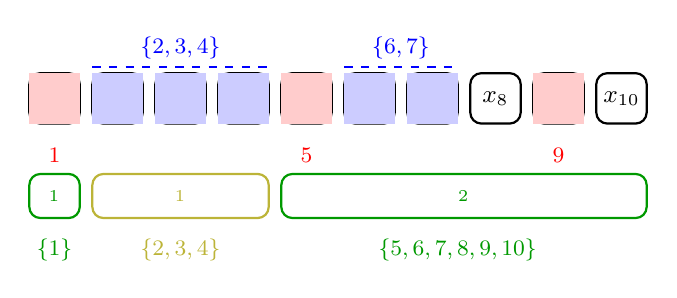
\begin{tikzpicture}[scale=0.8, every node/.style={align=center, font=\small}]
        % Draw the sequence of tokens
        \foreach \i in {1, 2, 3, 4, 5, 6, 7, 8, 9, 10} {
            \draw[rounded corners, thick] (\i, 0) rectangle (\i+0.8, 0.8) node[pos=.5] {$x_{\i}$};
        }

        % Highlight previously sampled tokens (M_<i)
        \foreach \i in {2, 3, 4, 6, 7} {
            \fill[blue!20] (\i, 0) rectangle (\i+0.8, 0.8);
        }

        % Highlight contiguous segments in M_<i
        \draw[thick, dashed, blue] (2, 0.9) -- (4.8, 0.9); % First segment: {2, 3, 4}
        \node[blue] at (3.4, 1.2) {\footnotesize $\{2, 3, 4\}$};

        \draw[thick, dashed, blue] (6, 0.9) -- (7.8, 0.9); % Second segment: {6, 7}
        \node[blue] at (6.9, 1.2) {\footnotesize $\{6, 7\}$};

        % Highlight current sampled tokens (M_i)
        \foreach \i in {1, 5, 9} {
            \fill[red!20] (\i, 0) rectangle (\i+0.8, 0.8);
        }

        % Label current tokens
        \node[red] at (1.4, -0.5) {\footnotesize $1$};
        \node[red] at (5.4, -0.5) {\footnotesize $5$};
        \node[red] at (9.4, -0.5) {\footnotesize $9$};

        % Draw intervals
        \draw[thick, green!60!black, rounded corners] (1, -1.5) rectangle (1.8, -0.8) node[pos=.5] {\small $\gI_1$};
        \node[green!60!black] at (1.4, -2) {\footnotesize $\{1\}$};

        \draw[thick, green!60!black, rounded corners] (5, -1.5) rectangle (10.8, -0.8) node[pos=.5] {\small $\gI_2$};
        \node[green!60!black] at (7.8, -2) {\footnotesize $\{5, 6, 7, 8, 9, 10\}$};

        \draw[thick, yellow!70!black, rounded corners] (2, -1.5) rectangle (4.8, -0.8) node[pos=.5] {\small $\gS_1$};
        \node[yellow!70!black] at (3.4, -2) {\footnotesize $\{2,3,4\}$};
    \end{tikzpicture}
    \caption{Illustration of the example for computing dependencies in the $n$-gram setting. Tokens $x_2, x_3, x_4, x_6, x_7$ (blue) represent the previously sampled location set $\gM_{<i}$, forming two contiguous segments: $\{2, 3, 4\}$ and $\{6, 7\}$. The current sampled locations $x_1, x_5, x_9$ (red) overlap with disjoint intervals $\gI_1 = \{1\}$ and $\gI_2 = \{5, 6, 7, 8, 9, 10\}$. The number of dependencies is computed as $\DEP_n(\gM_i, \gM_{<i}) = |\gM_i| - \text{(number of overlapping intervals)} = 3 - 2 = 1$.}
    \label{fig:dependencies}
\end{figure}


\noindent This example demonstrates how dependencies are computed, highlighting the interaction between previously sampled locations and the current reverse step. Such formalization is critical for understanding the efficiency and accuracy of discrete diffusion processes.

Finally, we extend this concept to define the total number of dependencies across an entire reverse process:

\begin{definition}[Number of Dependencies in a Reverse Process]
    Consider a reverse process $\tau = (\gM_1, \gM_2, \dots, \gM_N)$. Under the $n$-gram setting, the total number of dependencies in the process is defined as the sum of the dependencies across all steps:
    \[
    \DEP_n(\tau) = \sum_{i=1}^N \DEP_n(\gM_i, \gM_{<i}).
    \]
\end{definition}

Using the definition of $\DEP_n(\tau)$, we can bound the KL divergence between the distribution of sequences sampled under an instance of the reverse process and the ground-truth distribution in the $n$-gram setting.

\begin{lemma}[KL Divergence Upper Bound for the Instance of Reverse Process]
\label{lemma:kl_upper_ins_rev}
    Let $q$ denote the data distribution for sequences of length $L$, and let $p$ denote the distribution of sequences of length $L$ generated by reverse model $p_\theta$ via the reverse process $\tau$. Under \cref{ass:perfect_learning}, the following upper bound holds:
    \[
    \DKL{q}{p(\cdot|\tau)} \leq \DEP_n(\tau) \log |\gV|+L\eps_\mathrm{learning},
    \]
    where $\gV$ denote the vocabulary.
\end{lemma}

\begin{proof}
    Using \cref{lemma:kl_decomp_rev}, we have:
    $$\DKL{q}{p_\tau} = \sum_{i=1}^N \mathbb{E}_{\Tilde{\vx}_{<i}}\DKL{q(\Tilde{\vx}_i | \Tilde{\vx}_{<i})}{p_\tau(\Tilde{\vx}_i | \Tilde{\vx}_{<i})}.$$
    For each time step $t_i$:
    $$\mathbb{E}_{\Tilde{\vx}_{<i}}\DKL{q(\Tilde{\vx}_i | \Tilde{\vx}_{<i})}{p_\tau(\Tilde{\vx}_i | \Tilde{\vx}_{<i})}=\mathbb{E}_{\Tilde{\vx}_{<i}}\sum_{\Tilde{\vx}_i\in\gV^{|\gM_i|}}q(\Tilde{\vx}_i | \Tilde{\vx}_{<i})\log\frac{q(\Tilde{\vx}_i | \Tilde{\vx}_{<i})}{p_\tau(\Tilde{\vx}_i | \Tilde{\vx}_{<i})}.$$
    Given $\gM_i$ and $\gM_{<i}$, the tokens $\Tilde{\vx}_i$ at step $t_i$ can be partitioned into independently sampled token sets $\Tilde{\vx}_i^{(1)},\cdots,\Tilde{\vx}_i^{(m)}$ with $k_j$ denoting the size of each token set: 
    $$k_j=|\Tilde{\vx}_i^{(j)}|,\ j\in[m],\quad m=|\gM_i|-\DEP_n(\gM_i,\gM_{<i}).$$
    Using the independence, for each $\Tilde{\vx}_{<i}$, we can decompose the sum into:
    \begin{align*}
    \sum_{\Tilde{\vx}_i\in\gV^{|\gM_i|}}q(\Tilde{\vx}_i | \Tilde{\vx}_{<i})\log\frac{q(\Tilde{\vx}_i | \Tilde{\vx}_{<i})}{p_\tau(\Tilde{\vx}_i | \Tilde{\vx}_{<i})}&=\sum_{j=1}^m\sum_{\Tilde{\vx}_i^{(j)}\in\gV^{k_j}}q(\Tilde{\vx}_i^{(j)} | \Tilde{\vx}_{<i})\log\frac{q(\Tilde{\vx}_i^{(j)} | \Tilde{\vx}_{<i})}{p_\tau(\Tilde{\vx}_i^{(j)} | \Tilde{\vx}_{<i})}\\
    &=\sum_{j=1}^m\DKL{q(\Tilde{\vx}_i^{(j)} | \Tilde{\vx}_{<i})}{p_\tau(\Tilde{\vx}_i^{(j)} | \Tilde{\vx}_{<i}}.
    \end{align*}
    Under \cref{ass:perfect_learning}, the KL divergence between $q$ and $p_\theta$ is bounded by:
    $$\DKL{q_{0|t}(x_0^i \mid \vx_t)}{p_\mathbf{\theta}(x_0^i \mid \vx_t)} < \epsilon_\text{learning}, \quad \forall\ t \text{ and } \vx_t.$$
    By \cref{lemma:kl_mul_token_sample}, we know that:
    $$\DKL{q(\Tilde{\vx}_i^{(j)} | \Tilde{\vx}_{<i})}{p_\tau(\Tilde{\vx}_i^{(j)} | \Tilde{\vx}_{<i}}\leq (k_j-1)\log|\gV|+k_j\eps_\mathrm{learning}.$$
    Substituting back:
    $$\sum_{\Tilde{\vx}_i\in\gV^{|\gM_i|}}q(\Tilde{\vx}_i | \Tilde{\vx}_{<i})\log\frac{q(\Tilde{\vx}_i | \Tilde{\vx}_{<i})}{p_\tau(\Tilde{\vx}_i | \Tilde{\vx}_{<i})}\leq\sum_{j=1}^m(k_j-1)\log|\gV|+k_j\eps_\mathrm{learning}.$$
    Using the fact that
    $$\sum_{j=1}^m(k_j-1)=|\gM_i|-m=\DEP_n(\gM_i,\gM_{<i}),\quad \sum_{j=1}^mk_j=|\gM_i|$$
    we can obtain:
    $$\mathbb{E}_{\Tilde{\vx}_{<i}}\DKL{q(\Tilde{\vx}_i | \Tilde{\vx}_{<i})}{p_\tau(\Tilde{\vx}_i | \Tilde{\vx}_{<i})}\leq \DEP_n(\gM_i,\gM_{<i})\log|\gV|+|\gM_i|\eps_\mathrm{learning}.$$
    Thus, combined with the definition of $\DEP_n(\tau)$ and $p_\tau=p(\cdot|\tau)$, we can draw the final conclusion:
    \begin{align*}
        \DKL{q}{p(\cdot|\tau)} &\leq \sum_{i=1}^N\left(\DEP_n(\gM_i,\gM_{<i})\log|\gV|+|\gM_i|\eps_\mathrm{learning}\right)\\
        &=\DEP_n(\tau) \log |\gV|+L\eps_\mathrm{learning}.
    \end{align*}
    %In other words:
    %$$\DKL{q}{p(\cdot|\tau)} = \sum_{i=1}^N \DKL{q(\Tilde{\vx}_i | \Tilde{\vx}_{<i})}{p_\tau(\Tilde{\vx}_i | \Tilde{\vx}_{<i})}.$$
\end{proof}

The above Lemma directly leads to the bound for the KL divergence between the distribution of sequences generated by the reverse model with a given masking schedule and the ground-truth distribution in the $n$-gram setting.

\begin{lemma}[KL Divergence Upper Bound for a Masking Schedule]
\label{lemma:kl_bound_mask}
    Let $q$ denote the data distribution over sequences of length $L$, and let $p$ denote the distribution over sequences of length $L$ generated by the reverse model $p_\theta$ with masking schedule $\alpha_t$ and $N$ reverse steps. Under \cref{ass:perfect_learning}, the KL divergence between $q$ and $p$ satisfies the following upper bound:
    \[
    \DKL{q}{p} \leq \log |\gV| \sum_{i=1}^N \E_{\tau\sim\PROC(L, \alpha_t, N)} \DEP_n(\gM_i, \gM_{<i})+L\eps_\mathrm{learning}.
    \]
\end{lemma}

\begin{proof}
    By \cref{lemma:kl_upper_mask}, we can obtain:
    $$\DKL{q}{p} \leq \mathbb{E}_{\tau \sim \PROC(\alpha_t, N, L)} \DKL{q}{p(\cdot | \tau)}.$$
    Applying \cref{lemma:kl_upper_ins_rev} to the instances of reverse process, we can conclude that:
    \begin{align*}
    \DKL{q}{p} &\leq \mathbb{E}_{\tau \sim \PROC(\alpha_t, N,L)}\sum_{i=1}^N\DEP_n(\gM_i,\gM_{<i})\log|\gV|+L\eps_\mathrm{learning}\\
    &=\log |\gV| \sum_{i=1}^N \E_{\tau\sim\PROC(L, \alpha_t, N)} \DEP_n(\gM_i, \gM_{<i})+L\eps_\mathrm{learning}.
    \end{align*}
\end{proof}

For the final estimation, we need to derive an upper bound for the expected number of dependencies at each reverse step. First, we use Chernoff Bound to control the number of separators and new locations at each reverse step for a given masking schedule.

\begin{lemma}[Bounds on Separator and New Location Count at Each Reverse Step]
\label{lemma:bound_sep_new_rev}
    Given a sequence of length $L$, a masking schedule $\alpha_t$, and $N$ reverse steps. Assume that $L$ is divisible by $n-1$. Given the time step $t_i = \frac{N-i}{N}$, let $\NEW$ denote the number of locations sampled at step $t_i$, and $\SEP_n$ denote the number of separators in the previously sampled locations. Under the $n$-gram setting, the following bounds hold for $\NEW$ and $\SEP_n$:
    \begin{align*}
        \Pr\left(\SEP_n\leq \frac{Lp_i^{n-1}}{2(n-1)}\right)&\leq e^{-\frac{Lp_i^{n-1}}{8(n-1)}},\\
        \Pr\left(\NEW\geq 2L\delta_i\right)&\leq e^{-\frac{L\delta_i}{3}},
    \end{align*}
    where $p_i = \alpha_{t_{i-1}}$ and $\delta_i = \alpha_{t_i} - \alpha_{t_{i-1}}$.
\end{lemma}

\begin{proof}
Given a masking schedule $\alpha_t$, using the expression of true reverse process in \cref{eq:rev_proc} and $\alpha_1=0$, we can compute the probability $p^{(i)}$ of a token being sampled at time step $t_i$ to be:
$$p^{(i)}=\frac{\alpha_{t_i}-\alpha_{t_{i-1}}}{1-\alpha_{t_{i-1}}}\cdot\prod_{j=1}^{i-1}\frac{1-\alpha_{t_j}}{1-\alpha_{t_{j-1}}}=\alpha_{t_i} - \alpha_{t_{i-1}}=\delta_i.$$
Therefore, $\delta_i$ is the probability of a location being sampled at time step $t_i$. Summing up $\delta_i$, we can know that $p_i=\sum_{j=1}^{i-1}\delta_j$ is the probability of a location being sampled prior to time step $t_i$.

To derive a bound for $\SEP_n$, we partition the sequence into $\frac{L}{n-1}$ intervals, each of length $n-1$. For a given interval, the probability that all locations within the interval have been sampled prior to step $t_i$ is $p_i^{n-1}$. Define $X_j=1$ if the locations in the $j$-th interval have been sampled prior to $t_i$, and $X_j=0$ otherwise. The random variables $X_1,X_2,\cdots,X_{\frac{L}{n-1}}$ are independent and satisfy the following expectation:
$$\mathbb{E}_{\tau \sim \PROC(L, \alpha_t, N)}\sum_{j=1}^{\frac{L}{n-1}}X_j=\frac{Lp_i^{n-1}}{n-1}.$$
By the definition of $\SEP_n$, we know that:
$$\SEP_n\geq\sum_{j=1}^{\frac{L}{n-1}}X_j.$$
Applying \cref{lemma:chernoff} to the sum of $X_j$, we derive:
$$\Pr\left(\SEP_n\leq \frac{Lp_i^{n-1}}{2(n-1)}\right)\leq \Pr\left(\sum_{j=1}^{\frac{L}{n-1}}X_j\leq \frac{Lp_i^{n-1}}{2(n-1)}\right)\leq e^{-\frac{Lp_i^{n-1}}{8(n-1)}}.$$

Next, we consider the bound for $\NEW$. Given that the sequence contains $L$ locations and the probability of sampling any specific location at step $t_i$ is $\delta_i$, the expected number of new locations sampled at $t_i$ is given by:
$$\mathbb{E}_{\tau \sim \PROC(L, \alpha_t, N)}\NEW=L\delta_i.$$
Since the sampling of each location occurs independently, applying \cref{lemma:chernoff}, we have:
$$\Pr\left(\NEW\geq 2L\delta_i\right)\leq e^{-\frac{L\delta_i}{3}}.$$
\end{proof}

Using the above lemma, we can divide the estimation for the number of dependencies into three cases, and derive the bound case by case. This is achieved by using a variety of means and careful estimations.

\begin{lemma}[Upper Bound for the Expectation of Dependencies at Each Reverse Step]
\label{lemma:bound_dep_rev}
    Given a sequence of length $L$, a masking schedule $\alpha_t$, and $N$ reverse steps. Assume $L\delta_i>1$, then the expected number of dependencies at time step $t_i = \frac{N-i}{N}$ satisfies:
    \[
    \mathbb{E}_{\tau \sim \PROC(L, \alpha_t, N)} \DEP_n(\gM_i, \gM_{<i}) \leq \frac{9}{3+L\delta_i}+\frac{C(n-1)L\delta_i^2}{p_i^{n-1}},
    \]
    where $p_i = \alpha_{t_{i-1}}$, $\delta_i = \alpha_{t_i} - \alpha_{t_{i-1}}$, and $C$ is a constant.
\end{lemma}

\begin{proof}
By \cref{lemma:bound_sep_new_rev}, at step $t_i$, the following bounds hold:
\begin{align*}
        \Pr\left(\SEP_n\leq \frac{Lp_i^{n-1}}{2(n-1)}\right)&\leq e^{-\frac{Lp_i^{n-1}}{8(n-1)}},\\
        \Pr\left(\NEW\geq 2L\delta_i\right)&\leq e^{-\frac{L\delta_i}{3}}.
\end{align*}
Since $\DEP_n(\gM_i, \gM_{<i})\geq 0$, its expectation can be decomposed into three components:
\begin{align*}
    \mathbb{E}_{\tau \sim \PROC(L, \alpha_t, N)} \DEP_n(\gM_i, \gM_{<i})&=\Pr\left(\NEW\geq 2L\delta_i\right)\cdot \mathbb{E}_{\substack{\tau \sim \PROC(L, \alpha_t, N)\\ \NEW\geq 2L\delta_i}} \DEP_n(\gM_i, \gM_{<i})&\textbf{(Case 1)}\\
    &+\Pr\left(\SEP_n\leq \frac{Lp_i^{n-1}}{2(n-1)},\ \NEW< 2L\delta_i\right)\cdot \\
    &\qquad\mathbb{E}_{\substack{\tau \sim \PROC(L, \alpha_t, N)\\ \SEP_n\leq \frac{Lp_i^{n-1}}{2(n-1)}\\ \NEW< 2L\delta_i}} \DEP_n(\gM_i, \gM_{<i}) &\textbf{(Case 2)}\\
    &+\Pr\left(\SEP_n>\frac{Lp_i^{n-1}}{2(n-1)},\ \NEW< 2L\delta_i\right)\cdot \\
    &\qquad\mathbb{E}_{\substack{\tau \sim \PROC(L, \alpha_t, N)\\ \SEP_n>\frac{Lp_i^{n-1}}{2(n-1)}\\ \NEW<2L\delta_i}} \DEP_n(\gM_i, \gM_{<i})&\textbf{(Case 3)}
\end{align*}
We estimate these three cases separately.

\textbf{Case 1:} $\NEW\geq 2L\delta_i$.

By the definitions of $\DEP_n(\gM_i, \gM_{<i})$ and $\NEW$, we have:
$$\DEP_n(\gM_i, \gM_{<i})\leq |\gM_i|=\NEW.$$
Substituting this into the estimation, we obtain:
$$\Pr\left(\NEW\geq 2L\delta_i\right)\cdot \mathbb{E}_{\substack{\tau \sim \PROC(L, \alpha_t, N)\\ \NEW\geq 2L\delta_i}} \DEP_n(\gM_i, \gM_{<i})\leq \Pr\left(\NEW\geq 2L\delta_i\right)\cdot \mathbb{E}_{\substack{\tau \sim \PROC(L, \alpha_t, N)\\ \NEW\geq 2L\delta_i}} \NEW$$
Since $\DEP_n(\gM_i, \gM_{<i})\geq 0$, the expectation can be expressed as an integral of the tail probability:
$$\mathbb{E}_{\substack{\tau \sim \PROC(L, \alpha_t, N)\\ \NEW\geq 2L\delta_i}} \NEW=\int_{2L\delta_i}^{+\infty} \Pr\left(\NEW\geq x\mid\NEW\geq 2L\delta_i\right)\dd x.$$
It directly follows that:
\begin{align*}
    \Pr\left(\NEW\geq 2L\delta_i\right)\cdot \mathbb{E}_{\substack{\tau \sim \PROC(L, \alpha_t, N)\\ \NEW\geq 2L\delta_i}} \NEW &=\Pr\left(\NEW\geq 2L\delta_i\right)\cdot \int_{2L\delta_i}^{+\infty} \Pr\left(\NEW\geq x\mid\NEW\geq 2L\delta_i\right)\dd x\\
    &=\int_{2L\delta_i}^{+\infty} \Pr\left(\NEW\geq x\mid\NEW\geq 2L\delta_i\right)\Pr\left(\NEW\geq 2L\delta_i\right)\dd x\\
    &=\int_{2L\delta_i}^{+\infty}\Pr\left(\NEW\geq x\right)\dd x.
\end{align*}
Using the same trick as \cref{lemma:bound_sep_new_rev}, applying \cref{lemma:chernoff}, we can derive the bound for probability $\Pr\left(\NEW\geq x\right)$ as:
$$\Pr\left(\NEW\geq x\right)\leq e^{-\frac{(x-L\delta_i)^2}{x+L\delta_i}}.$$
Note that $\NEW\leq L$, we only need to consider $2\delta_i\leq 1$. In this case, we have:
\begin{align*}
    \int_{2L\delta_i}^{+\infty}\Pr\left(\NEW\geq x\right)\dd x \leq \int_{2L\delta_i}^{L}e^{-\frac{(x-L\delta_i)^2}{x+L\delta_i}}\dd x
\end{align*}
Let $y=x-L\delta_i\in[L\delta_i,L(1-\delta_i)]$, the integral can be rewritten as:
$$\int_{2L\delta_i}^{+\infty}\Pr\left(\NEW\geq x\right)\dd x \leq \int_{L\delta_i}^{L(1-\delta_i)}e^{-\frac{y^2}{y+2L\delta_i}}\dd y.$$
Observe that $y+2L\delta_i\leq 3y$, we can obtain:
$$\int_{2L\delta_i}^{+\infty}\Pr\left(\NEW\geq x\right)\dd x \leq \int_{L\delta_i}^{L(1-\delta_i)}e^{-\frac{y^2}{3y}}\dd y =3\left(e^{-\frac{L\delta_i}{3}}-e^{-\frac{L(1-\delta_i)}{3}}\right)=3e^{-\frac{L\delta_i}{3}}\left(1-e^{-\frac{L(1-2\delta_i)}{3}}\right).$$
Using the fact that $e^{-x}\leq\frac{1}{1+x}$ for $x\geq 0$, we have the upper bound:
$$3e^{-\frac{L\delta_i}{3}}\left(1-e^{-\frac{L(1-2\delta_i)}{3}}\right)\leq 3e^{-\frac{L\delta_i}{3}}\leq \frac{9}{3+L\delta_i}.$$
Combining the above results, we know that:
$$\Pr\left(\NEW\geq 2L\delta_i\right)\cdot \mathbb{E}_{\substack{\tau \sim \PROC(L, \alpha_t, N)\\ \NEW\geq 2L\delta_i}} \DEP_n(\gM_i, \gM_{<i})\leq \frac{9}{3+L\delta_i}.$$

\textbf{Case 2:} $\SEP_n\leq \frac{Lp_i^{n-1}}{2(n-1)}$ and $ \NEW<2L\delta_i$.

Similar to Case 1, we have:
$$\DEP_n(\gM_i, \gM_{<i})\leq\NEW<2L\delta_i,$$
so the expectation also follows:
$$\mathbb{E}_{\substack{\tau \sim \PROC(L, \alpha_t, N)\\ \SEP_n\leq \frac{Lp_i^{n-1}}{2(n-1)}\\ \NEW< 2L\delta_i}} \DEP_n(\gM_i, \gM_{<i})< 2L\delta_i.$$
Using the probability bound, it follows that:
$$\Pr\left(\SEP_n\leq \frac{Lp_i^{n-1}}{2(n-1)},\ \NEW< 2L\delta_i\right)\leq\Pr\left(\SEP_n\leq \frac{Lp_i^{n-1}}{2(n-1)}\right)\leq e^{-\frac{Lp_i^{n-1}}{8(n-1)}}.$$
Since $e^{-x}\leq\frac{1}{1+x}$ for $x\geq 0$:
$$e^{-\frac{Lp_i^{n-1}}{8(n-1)}}\leq\frac{8(n-1)}{Lp_i^{n-1}+8(n-1)}.$$
Combining these results, we obtain:
$$\Pr\left(\SEP_n\leq \frac{Lp_i^{n-1}}{2(n-1)},\ \NEW< 2L\delta_i\right)\cdot\mathbb{E}_{\substack{\tau \sim \PROC(L, \alpha_t, N)\\ \SEP_n\leq \frac{Lp_i^{n-1}}{2(n-1)}\\ \NEW< 2L\delta_i}} \DEP_n(\gM_i, \gM_{<i})\leq \frac{16(n-1)L\delta_i}{Lp_i^{n-1}+8(n-1)}.$$

\textbf{Case 3:} $\SEP_n>\frac{Lp_i^{n-1}}{2(n-1)}$ and $ \NEW<2L\delta_i$.

Apparently, we have:
$$\Pr\left(\SEP_n>\frac{Lp_i^{n-1}}{2(n-1)},\ \NEW< 2L\delta_i\right)\leq 1.$$
Given $a,b$, let $\mathbb{E}_{a,b}\DEP_n(\gM_i, \gM_{<i})$ denote the expectation of $\DEP_n(\gM_i, \gM_{<i})$ under the condition of $\SEP_n=a$ and $ \NEW=b$. In other words:
$$\mathbb{E}_{a,b}\DEP_n(\gM_i, \gM_{<i})=\mathbb{E}_{\substack{\tau \sim \PROC(L, \alpha_t, N)\\ \SEP_n=a\\ \NEW=b}} \DEP_n(\gM_i, \gM_{<i}).$$
Since all the locations are sampled independently, and $\DEP_n(\gM_i, \gM_{<i})$ depends only on the relative positions of separators in $\gM_{<i}$ and the new locations in $\gM_i$, the expectation $\mathbb{E}_{a,b}\DEP_n(\gM_i, \gM_{<i})$ only depends on the ordering of separators and new locations.

Assume $x_1,\cdots,x_{a+b}$ are $a+b$ positions (not locations) in order. We can regard the process of ordering separators and new locations as the process of choosing $b$ positions randomly from $x_j$. For $1\leq j\leq a+b-1$, define $X_j=1$ if $x_j$ and $x_{j+1}$ are both new locations, and $X_j=0$ otherwise. By the definition of $\DEP_n(\gM_i, \gM_{<i})$, we can obtain:
$$\DEP_n(\gM_i, \gM_{<i})=\sum_{j=1}^{a+b-1}X_j.$$
Since the $b$ new locations are chosen randomly, the probability of $X_j=1$ can be calculated as:
$$\Pr(X_j=1)=\frac{C_{a+b-2}^{b-2}}{C_{a+b}^{b}}=\frac{b(b-1)}{(a+b)(a+b-1)}.$$
Therefore, the expectation of $X_j$ is:
$$\mathbb{E}X_j=\frac{b(b-1)}{(a+b)(a+b-1)}.$$
Summing up, we have:
$$\mathbb{E}_{a,b}\DEP_n(\gM_i, \gM_{<i})=\mathbb{E}\sum_{j=1}^{a+b-1}X_j=(a+b-1)\mathbb{E}X_1=\frac{b(b-1)}{a+b}.$$
Since $a>\frac{Lp_i^{n-1}}{2(n-1)}$ and $b<2L\delta_i$, we can derive the upper bound for any $a,b$:
$$\frac{b(b-1)}{a+b}\leq \frac{b(b-1)}{\frac{Lp_i^{n-1}}{2(n-1)}+b} \leq\frac{2L\delta_i(2L\delta_i-1)}{\frac{Lp_i^{n-1}}{2(n-1)}+2L\delta_i}\leq \frac{8(n-1)L\delta_i^2}{p_i^{n-1}+4(n-1)\delta_i}.$$
Since this holds for all $a$ and $b$, we can obtain:
\begin{align*}
    &\quad\Pr\left(\SEP_n>\frac{Lp_i^{n-1}}{2(n-1)},\ \NEW< 2L\delta_i\right)\cdot\mathbb{E}_{\substack{\tau \sim \PROC(L, \alpha_t, N)\\ \SEP_n>\frac{Lp_i^{n-1}}{2(n-1)}\\ \NEW<2L\delta_i}} \DEP_n(\gM_i, \gM_{<i})\\
    &\leq \mathbb{E}_{\substack{\tau \sim \PROC(L, \alpha_t, N)\\ \SEP_n>\frac{Lp_i^{n-1}}{2(n-1)}\\ \NEW<2L\delta_i}} \DEP_n(\gM_i, \gM_{<i})\\
    &=\sum_{a>\frac{Lp_i^{n-1}}{2(n-1)},\ b<2L\delta_i}\Pr(\SEP_n=a, \NEW=b)\cdot\mathbb{E}_{a,b}\DEP_n(\gM_i, \gM_{<i})\\
    &\leq \frac{8(n-1)L\delta_i^2}{p_i^{n-1}+4(n-1)\delta_i}.
\end{align*}

\textbf{Summarize the above proof:}

Combining the above three cases, we can obtain:
$$\mathbb{E}_{\tau \sim \PROC(L, \alpha_t, N)} \DEP_n(\gM_i, \gM_{<i}) \leq \frac{9}{3+L\delta_i}+\frac{16(n-1)L\delta_i}{Lp_i^{n-1}+8(n-1)}+\frac{8(n-1)L\delta_i^2}{p_i^{n-1}+4(n-1)\delta_i}.$$
If we have the assumption $L\delta_i\geq 1$, it is easy to find that:
\begin{align*}
    \mathbb{E}_{\tau \sim \PROC(L, \alpha_t, N)} \DEP_n(\gM_i, \gM_{<i}) &\leq \frac{9}{3+L\delta_i}+\frac{16(n-1)\delta_i}{p_i^{n-1}}+\frac{8(n-1)L\delta_i^2}{p_i^{n-1}}\\
    &\leq \frac{9}{3+L\delta_i}+\frac{16(n-1)L\delta_i^2}{p_i^{n-1}}+\frac{8(n-1)L\delta_i^2}{p_i^{n-1}}\\
    &\leq \frac{9}{3+L\delta_i}+\frac{C(n-1)L\delta_i^2}{p_i^{n-1}}.
\end{align*}
Where $C=24$ is a constant.

\end{proof}

Finally, we can derive the upper bound for the KL divergence between the distribution of sequences generated by the
reverse model and the ground-truth distribution in the n-gram setting.

\begin{lemma}[Efficient Sampling with Small KL Divergence]
\label{lemma:effi_kl_bound}
    Let $q$ denote the data distribution over sequences of length $L$, and let $p$ denote the distribution over sequences of length $L$ generated by the reverse model $p_\theta$ with a masking schedule $\alpha_t$ and $N$ reverse steps. Assume that $p_\theta$ satisfies \cref{ass:perfect_learning}. For any $\epsilon > 0$, there exists a masking schedule $\alpha_t$ such that, for $L\geq \frac{3C(n-1)}{\eps^{n+\frac{1}{2}}}$, with $N = O\left(\frac{n-1}{\eps^{n}}\right)$ sampling steps, the KL divergence between $q$ and $p$ satisfies:
    $$\frac{\DKL{q}{p}}{L\log|\gV|} \leq 4\eps +\frac{\eps_\mathrm{learning}}{\log|\gV|}.$$
\end{lemma}

\begin{proof}
    By \cref{lemma:kl_bound_mask}, we know that:
    $$\DKL{q}{p} \leq \log |\gV| \sum_{i=1}^N \E_{\tau\sim\PROC(L, \alpha_t, N)} \DEP_n(\gM_i, \gM_{<i})+L\eps_\mathrm{learning}.$$
    Note that at step $t_1$, the reverse process can be bounded using \cref{lemma:kl_mul_token_sample}. By reviewing our proof process, it is easy to see that we can substitute $\DEP_n(\gM_1, \gM_{<1})$ for $(|\gM_1|-1)\log |\gV|$, where $\gV$ stands for the vocabulary. By the definition of $\delta_i$, we know that:
    $$\E_{\tau\sim\PROC(L, \alpha_t, N)} (|\gM_1|-1)\log |\gV|=(\delta_1L-1)\log |\gV|.$$
    Applying \cref{lemma:bound_dep_rev} to $\DEP_n(\gM_i, \gM_{<i})$, if $L\delta_i\geq 1$, we can obtain:
    $$\DKL{q}{p}\leq \delta_1\log |\gV|+\log |\gV| \sum_{i=2}^N\left(\frac{9}{3+L\delta_i}+\frac{C(n-1)L\delta_i^2}{p_i^{n-1}}\right)+L\eps_\mathrm{learning}.$$
    By the definition of $p_i$, we know that $p_2=\delta_1$. For any small $\eps>0$, consider the following masking schedule:
    %$$\delta_1=\frac{\eps}{\log |\gV|},\quad \delta_i=\delta=\frac{\eps^n}{C(n-1)(\log|\gV|)^n},\quad p_i=\delta_1+(i-2)\delta,\quad\forall i\geq 2.$$
    $$\delta_1=\eps,\quad \delta_i=\delta=\frac{\eps^n}{C(n-1)},\quad p_i=\delta_1+(i-2)\delta,\quad\forall i\geq 2.$$
    Then, for $L\geq \frac{1}{\delta}$, the KL divergence can be bounded by:
    \begin{align*}
        \frac{\DKL{q}{p}}{L\log|\gV|}&\leq \eps+\frac{9(N-1)}{L(3+L\delta)}+\sum_{i=2}^N \frac{C(n-1)\delta^2}{p_i^{n-1}}+\frac{\eps_\mathrm{learning}}{\log|\gV|}\\
        &=\eps+\frac{9(1-\delta_1)}{L\delta(3+L\delta)}+\frac{C(n-1)\delta^2}{\delta_1^{n-1}}+\sum_{i=1}^{N-2} \frac{C(n-1)\delta^2}{(\delta_1+i\delta)^{n-1}}+\frac{\eps_\mathrm{learning}}{\log|\gV|}.\\
        &\leq \eps+\frac{9}{L\delta(3+L\delta)}+\frac{C(n-1)\delta^2}{\delta_1^{n-1}}+\sum_{i=1}^{N-2} \frac{C(n-1)\delta^2}{(\delta_1+i\delta)^{n}}+\frac{\eps_\mathrm{learning}}{\log|\gV|}.
    \end{align*}
    By simple calculations, we know that:
    $$\frac{9}{L\delta(3+L\delta)}\leq \eps,\quad \text{if }L\geq \frac{3}{\delta\eps^{\frac{1}{2}}}.$$
    It is clear that $\delta\leq 1$, so:
    $$\frac{C(n-1)\delta^2}{\delta_1^{n-1}}\leq \eps\delta\leq\eps.$$
    Since $x^{-n}$ is convex on $[0,+\infty)$, the accumulation can be bounded by:
    \begin{align*}
        \sum_{i=1}^{N-2} \frac{C(n-1)\delta^2}{(\delta_1+i\delta)^n}&=C(n-1)\delta^{2-n}\sum_{i=1}^{N-2}\frac{1}{(\frac{\delta_1}{\delta}+i)^n}\\
        &\leq C(n-1)\delta^{2-n}\sum_{i=1}^{N-2}\int_{x=0}^{+\infty}\frac{1}{(\frac{\delta_1}{\delta}+x)^n\dd x}\\
        &=C(n-1)\delta^{2-n}\cdot\frac{1}{n-1}\left(\frac{\delta}{\delta_1}\right)^{n-1}\\
        &=\frac{C\delta}{\delta_1^{n-1}}\\
        &\leq\eps.
    \end{align*}
    Combining the above, we have:
    $$\frac{\DKL{q}{p}}{L\log|\gV|}\leq 4\eps+\frac{\eps_\mathrm{learning}}{\log|\gV|}.$$
    Meanwhile, the time step is limited by:
    $$N=1+\frac{1-\delta_1}{\delta}=O\left(\frac{n-1}{\eps^n}\right),$$
    and the lower bound for $L$:
    $$L\geq \frac{3}{\delta\eps^{\frac{1}{2}}}=\frac{3C(n-1)}{\eps^{n+\frac{1}{2}}}.$$

\end{proof}

Combining the above lemmas, we can prove \cref{thm:acceleration_ngram} by breaking the expression of $\log\PPL(p)$ into two parts.

\begin{theorem}[$\PPL$ Bounds for $n$-Gram Language Generation]
    For any $n$-gram language $q$ and any $\epsilon > 0$, let $p_\mathsf{\theta}$ denote the reverse model and $L$ denote the sequence length. The distribution over sequences generated by $p_\mathsf{\theta}$ is denoted as $p$. For any $L>O\big( \frac{n-1}{\epsilon^{n+0.5}}\big)$, under \cref{ass:perfect_learning}, there exists a masking schedule $\alpha_t$ such that, with $N = O\big( \frac{n-1}{\epsilon^n}\big)$ sampling steps, the perplexity of the MDM is upper-bounded by:
    $$\log\PPL(p) \leq \log\PPL(q) + \epsilon_\text{learning} + 4\epsilon\log |\gV|.$$
\end{theorem}

\begin{proof}
    By \cref{lemma:effi_kl_bound}, for any $L>O\big( \frac{n-1}{\epsilon^{n+0.5}}\big)$, there exists a masking schedule $\alpha_t$ with $N = O\big( \frac{n-1}{\epsilon^n}\big)$ sampling steps satisfying:
    $$\frac{\DKL{q}{p}}{L\log|\gV|} \leq 4\eps+\frac{\eps_\mathrm{learning}}{\log|\gV|}.$$
    In other words:
    $$\frac{1}{L}\mathbb{E}_{\vx \sim q}
    \log \frac{q(\vx)}{p(\vx)}\leq 4\eps\log|\gV|+\eps_\mathrm{learning}.$$
    By the definition of $\PPL$, we have:
    $$\log\PPL(p) = \mathbb{E}_{\vx \sim q} -\frac{\log p(\vx)}{|\vx|}=\frac{1}{L}\mathbb{E}_{\vx \sim q}\left(-\log q(\vx)+\log\frac{q(\vx)}{p(\vx)}\right).$$
    Note that:
    $$\log\PPL(q) = \mathbb{E}_{\vx \sim q} -\frac{\log q(\vx)}{|\vx|}=\frac{1}{L}\mathbb{E}_{\vx \sim q}-\log q(\vx).$$
    We can obtain:
    $$\log\PPL(p) \leq \log\PPL(q) + \epsilon_\text{learning} + 4\epsilon\log |\gV|.$$
\end{proof}
